\chapter{Bibliotecas Digitais e Interoperabilidade}
\label{cap:bibinterop}
Nesse capitulo será apresentados conceitos sobre bibliotecas digitais, uma das soluções encontradas para catalogação dos mecanismos formais de participação.

\section{Conceitos Básicos Sobre Bibliotecas Digitais}

Uma biblioteca digital não é simplesmente uma coleção digital com ferramentas para manutenção das informações. Uma biblioteca digital é composta por um ambiente que possui coleções, serviços e pessoas apoiando um ciclo de vida de disseminação, uso e preservação do dado, informação e conhecimento.

De fato, as bibliotecas digitais vêm ganhando destaque por serem capazes de agregar valor aos serviços providos pelas bibliotecas tradicionais (não virtuais). Mediante o uso de protocolos que garantem interoperabilidade (como o Z39.50\footnote{Disponível em \url{http://pt.wikipedia.org/wiki/Z39.50}.} e o OAI-PMH\footnote{Informações disponíveis em \url{http://www.openarchives.org/}.}) e de padrões para descrição de metadados estruturais, descritivos, administrativos e de preservação \cite{rodrigrues2003preservacao}, as bibliotecas digitais tornaram-se suporte essencial para armazenamento, indexação, recuperação e distribuição de objetos digitais pela Internet. De acordo com a definição provida pela ARL\footnote{ARL ou Association of Research Libraries é uma organização composta por inúmeras instituições de pesquisa na área de Ciência da Informação – principalmente Estados Unidos e Canadá –, cujo objetivo é promover pesquisas, recomendar padrões e integrar as instituições envolvidas. Mais informações podem ser encontradas no endereço http://www.arl.org/.}, uma biblioteca digital é uma entidade que possui as seguintes características: (i) serve a vários usuários; (ii) é dirigida à tecnologia; (iii) é interligada com outras bibliotecas; (iv) é universalmente acessível; (v) não é limitada à digitalização de objetos impressos existentes; e (vi) pode ser provida de conteúdos multimídia que existam apenas em um ambiente digital.

Por sua vez, bibliotecas digitais não são apenas bibliotecas com conteúdo definido, mas entidades que têm uma variedade de propósitos e funções, dentre eles: (i) preservar objetos de informação; (ii) implantar melhorias na acessibilidade de materiais informacionais; (iii) integrar vários formatos de informação, sejam eles textuais, imagens e vídeos numa única coleção; e (iv) prover ferramentas de educação. 
Os objetos comportados em bibliotecas digitais representam artefatos que podem ou não terem sido captados do mundo real e existem modelos estabelecidos para a definição desses artefatos, como a proposição feita por \cite{kuramoto2007bibliotecas}, e que está ilustrada na figura \ref{fig:compartefdigital}.

Segundo \cite{arms2000digital}, ele ressalta que uma biblioteca digital é tão boa quanto assim for a sua interface, pois ela melhora a comunicação e reduz o esforço necessário para compreender a organização estrutural e espacial dos conteúdos, localizar objetos digitais específicos no sistema e nas telas, além de proporcionar uma navegação fácil. 

\graphicspath{{figuras/}}
\begin{figure}[H]
\centering
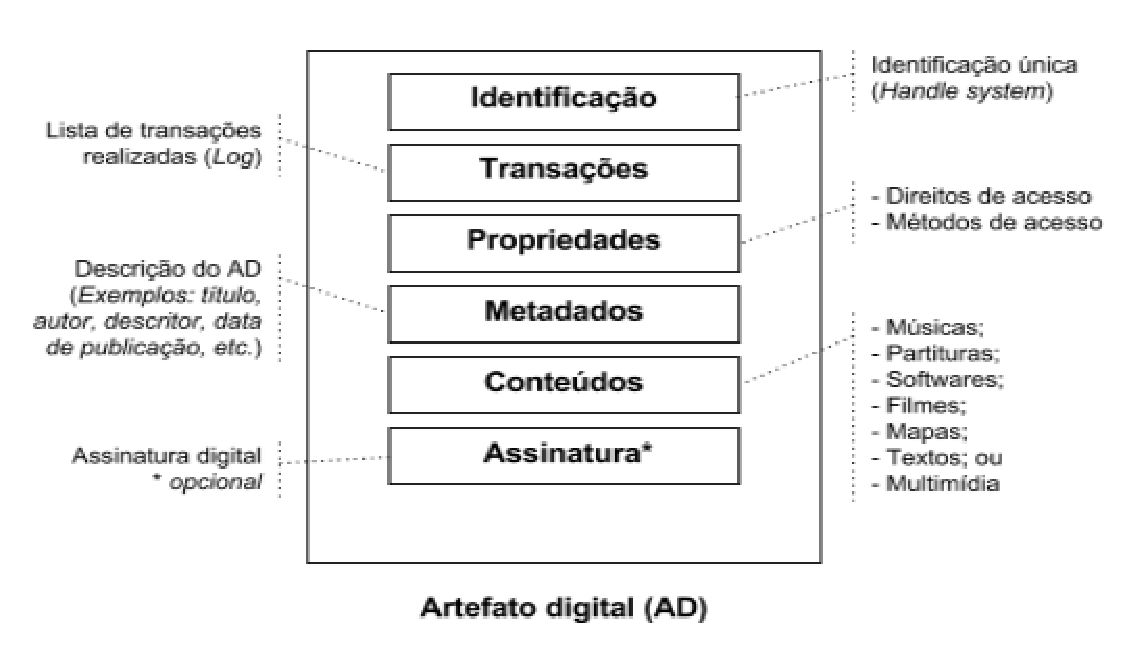
\includegraphics[width=0.8\textwidth]{artefato_digital}
\caption[Componentes de um artefato digital]{Componentes de um artefato digital. Adaptado de \cite{kuramoto2007bibliotecas}}
\label{fig:compartefdigital}
\end{figure}

Um objeto digital é a unidade básica de informação de uma biblioteca digital, em conjunto com os seus metadados e demais atributos, conforme está descrito na Figura \ref{fig:compartefdigital}.

Ainda de acordo com a figura \ref{fig:compartefdigital}, os artefatos digitais devem possuir: (i) uma assinatura digital como forma de certificação do produto; (ii) uma identificação do tipo de conteúdo que possui; (iii) os metadados descritivos, estruturais e administrativos; (iv) os direitos de acesso; (v) um controle de acessos e, finalmente (vi) uma identificação única. Abaixo é descrito cada um desses componentes: 

\begin{itemize}
	\item \textbf{Identificação} - Cada item tem que possui um identificador único, que é uma propriedade que distingue um objeto dos demais. Esse identificador pode ser um campo incremental, algum número de identificação único (CPF ou CNPJ), as iniciais do artefato (\textit{slugs}), entre outros.	
	\item \textbf{Transações} - É responsável por identificar e guardar em um arquivo de \textit{log} (registros), número de acessos a determinado artefato digital, quais itens do artefato digital foram acessados, etc.	
	\item \textbf{Propriedades} - Elas identificam quais são as diretivas de acesso para determinado artefato digital, no caso o artefato pode ser visualizado publicamente ou ter uma lista de determinados usuários que podem acessar o mesmo. Também identifica as  permissões de controle a esse item artefato (ler, editar, deletar). A propriedade identifica também qual será o caminho utilizado para se chegar a determinado artefato digital e como é feita a divisão do mesmo. Os métodos de acesso devem ser compatíveis com a forma de representação e devem atender a um público variado. Portanto, interfaces amigáveis (sistemas IHC – Interactive Human-Computer) para os diferentes tipos de usuário precisam ser contemplados.
	\item \textbf{Metadados} - Os metadados descrevem as características de um artefato digital \footnote{Visto mais detalhadamente adianta, na seção \ref{sec:padraometadado}}.	
	\item \textbf{Conteúdo} - O conteúdo é algo que faz parte de um artefato digital. Um artefato digital pode ser composto de vários tipos de conteúdo (áudio, vídeo, imagem, textos, etc.). 	
	\item \textbf{Assinatura} - A assinatura digital garante a autenticidade daquele artefato digital. Ele garante que o item acessado possui veracidade em suas informações, além de garantir também que as informações acessadas pelo usuários são integras (nada foi perdido).
\end{itemize}

Para uma prova de conceito da versão da biblioteca digital do Participa.br que será vista na subseção \ref{sub:prototipo_biblioteca}, a identificação é composta por um campo que auto incrementa a cada novo canal de participação cadastrado. As transações são compostas pelos \textit{logs} de acesso do próprio apache, que fornece os dados de acesso dos usuários \footnote{Os \textit{logs} do \textit{Apache} não fornece detalhes sobre os acessos sobre cada artefato digital, isso será implementado}. As propriedades de acesso definidas para os itens são (i) público - qualquer usuário pode acessar o item e (ii) privada - somente usuários permitidos em uma lista podem acessar o item.

Os Metadados serão explicados na subseção \ref{sub:metadadospbr}, onde será feita uma relação com os metadados DC, com os metadados do Participa.br. Em relação ao tipo de conteúdo, somente os no formato de texto digital(HMTL, TXT e PDF) foram relevados, no entanto, já foi levantado que existem conselhos e conferências que disponibilizam vídeos e áudios de suas reuniões. A assinatura digital não foi disponibilizada nessa primeira prova de conceito, já que serão feitas futuras reuniões com os gestores da SGPR com vistas de verificar a necessidade de implementação de assinaturas.

\section{Arquitetura das Bibliotecas Digitais}

De acordo com o que está apresentado na figura \ref{fig:modelbibdigital}, o projeto de interface é parte integrante do modelo conceitual do sistema, juntamente com o projeto funcional que especifica as funções a serem oferecidas aos usuários e ao projeto dos metadados associados aos dados que especificam a estrutura e a organização e descrição do conteúdo \cite[pp. 143--145]{arms2000digital}\cite[pp. 190]{ferreira2006interface}.

\graphicspath{{figuras/}}
\begin{figure}[H]
\centering
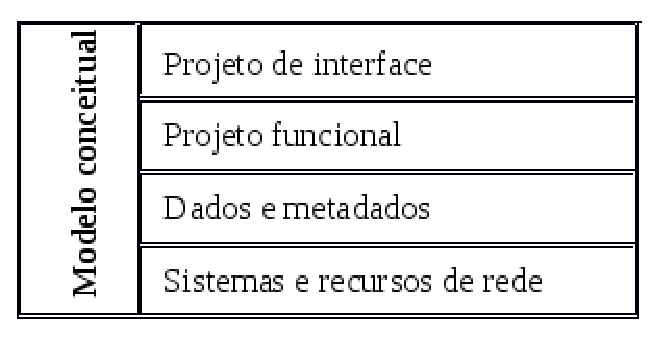
\includegraphics[width=0.5\textwidth]{modelo_biblioteca}
\caption[Modelo conceitual para projeto de bibliotecas digitais]{Modelo conceitual para projeto de bibliotecas digitais. Extraído de \cite[p. 144]{arms2000digital}}
\label{fig:modelbibdigital}
\end{figure}

Para o caso dos canais de participação social, esse modelo também pode ser usado como referência, dada a variedade de possibilidades de acesso, tipos de usuários e formas de representação dos artefatos digitais. Tais possibilidades impactam diretamente na construção das interfaces de acesso, dando origem a paradigmas que permitem expressões de busca diferenciadas.

Ainda de acordo com esse o modelo ilustrado pela figura \ref{fig:modelbibdigital} faz-se documentar todas as fases de implementação uma biblioteca completa. Apesar dessas documentação ficar escondida dos usuários, elas ajudam a criar um sistema com os módulos (busca, navegação, catalogação e demais) totalmente integrados, além de ajudar os usuários com uma sistema mais harmônico e robusto, consequentemente, tendo uma confiança na utilização do sistema pelo usuário. As figuras \ref{fig:sistemasoftware}  e \ref{fig:entregaveissoftware} representam os sistemas compostos pela arquitetura e os entregáveis de uma arquitetura, respectivamente.

\graphicspath{{figuras/}}
\begin{figure}[H]
\centering
\includegraphics[width=0.8\textwidth]{sistemas}
\caption[Identificação dos principais componentes de uma biblioteca]{Identificação dos principais componentes de um site. Adaptado de \cite{rosenfeld2002information}}
\label{fig:sistemasoftware}
\end{figure}

O diagrama ilustrado pela figura \ref{fig:sistemasoftware}, representa a arquitetura de informação utilizado em uma biblioteca. Se faz necessário ter uma documentação sobre a arquitetura de informação do sistema para os usuários terem um melhor entendimento, facilitando a interação do usuário com a biblioteca.

Um sistema de busca não é composto somente por uma interface bonita ou um bom motor de busca, mas por todo um conjunto integrado. O usuário tem que ser capaz de pesquisar qualquer tipo de conteúdo e ordena-lo conforme o seu gosto, e os resultados precisam ser apresentados de forma agradável. Portanto, na sua estrutura interna é preciso garantir que os resultados relativos a uma busca (expressa por um atributo de consulta, chamada de \textit{query}) sejam compatíveis com as demandas dos usuários e, ao mesmo tempo, que esses resultados sejam apresentados segundo uma ordem de importância e também de maneira agradável no sentido de interface. 

Para isso é necessário catalogar os artefatos digitais, pois definindo os metadados adequados facilitam o processo de busca. Adotando os padrões de metadados aceitos pela comunidade, como o Dublin Core, facilita a integração dessa biblioteca com outros contextos e sites de buscas, como é o caso do Google.

A ampliação do sistema para permitir um ambiente semântico permitem buscas mais refinadas, pois permitem que se façam inferências entre objetos correlatos e ajudam a máquina a entender as \textit{querys} dos usuários com mais facilidade. 

Além disso, também é necessário planejar todo o esquema de navegação e menus da biblioteca. Isso deixa a navegação mais ágil, facilitando a utilização do site pelo usuário.

\graphicspath{{figuras/}}
\begin{figure}[H]
\centering
\includegraphics[width=0.8\textwidth]{entregaveis}
\caption[Entregáveis de uma biblioteca]{Entregáveis de uma biblioteca. Adaptado de \cite{rosenfeld2002information}}
\label{fig:entregaveissoftware}
\end{figure}

A figura \ref{fig:entregaveissoftware} mostra os entregáveis de uma biblioteca, que são utilizados para um entendimento melhor do sistema a ser produzido. Esses entregáveis são compostos pelos (i)\textit{Blueprints}, também chamados de mapa do site são uma espécie do funcionamento de toda a arquitetura de informação presente no site. Eles mostram as relações de caminho entres as páginas e seus componentes. (ii) Os Wireframes descrevem uma página individual, mostrando todos os conteúdos e arquitetura da informação relacionados com a página através de um protótipo. Esse protótipo pode dizer quais informações podem ser informadas para o usuário e servir de insumo para o sistema final. (iii) Os vocabulários controlados permitem que um item seja encontrado através de palavras relacionadas, isso ajuda o cliente em interfaces de busca. Um exemplo de vocabulário controlado é um tesauro \footnote{Maiores informações em: \url{http://pt.wikipedia.org/wiki/Tesauro}}. (iv) O esquema de metadados, explicado mais detalhadamente na seção \ref{sec:padraometadado} ajudam a catalogar melhor os objetos digitais, fazendo com que a indexação de busca seja melhor.

Nesse primeiro trabalho, foram levantados alguns metadados com base no catálogo de mecanismos formais, disponível no Anexo \ref{Att:catalogomecanismos}. O produto de cada catalogação gerou um primeira versão do esquema de metadados, que é visto na seção \ref{cap:bibinterop}{sub:metadadospbr}. Apesar de não ser necessariamente um Wireframe, o primeiro protótipo da biblioteca digital de participação social visto na seção \ref{sub:prototipo_biblioteca} pode ser entendido como um, já que apresenta uma interface inicial onde há a exibição de conteúdos para os usuários.

\section{Padrões de Metadados para Catalogação e Sistematização de Dados}
\label{sec:padraometadado}

Na biblioteconomia, o metadado é dado estruturado que compartilha diversas características similares para a catalogação e descrevem as características de um determinado recurso informacional. Um registro de metadados consiste em um número predefinido de elementos que representam atributos específicos de um objeto e cada elemento pode estar associado a um ou mais valores. Os esquemas de metadados devem possuir (independente da área de conhecimento) um número limitado de elementos, o nome de cada elemento e o significado de cada elemento.

Dentre os benefícios de metadados na web, pode-se citar os seguintes: (i) são estruturados e formam a base para o desenvolvimento de sistemas de busca, (ii) podem ser convertidos para outros formatos, ou seja, interoperar com diferentes protocolos de busca e recuperação, (iii) tornam mais fácil a extração de conteúdo por engines de busca (SEOs) e (iv) facilitam o gerenciamento do sistema de informação (com os metadados administrativos) porque ajudam a avaliar quando os recursos devem ser revistos ou removidos da base de dados.

Em relação agrupamento dos elementos de metadados de um recursos computacional (classificação), podem ser classificados em:

\begin{itemize}
	\item \textbf{Descritivos} Passíveis de uso por sistemas de busca. Por exemplo o título, a descrição, URI, autor, idioma, formato de arquivo;
	\item \textbf{De assunto} (Relacionados à atividade de indexação) descrevem o conteúdo do documento, tais como as palavras-chave, os códigos e sistemas de classificação, termos do tesauro ou cabeçalho de assuntos; e
	\item \textbf{Administrativos} que facilitam a organização e administração do sistema de informação. Exemplos incluem o responsável pela manutenção do documento, data de adição do documento, data de expiração, dentre outros.
\end{itemize}

Do ponto de vista do grau de dificuldade de uso dos padrões, os metadados, podem ser classificados em formatos de bandas um, dois e três \cite{feitosa2006organizacao}. Os formatos de metadados de banda um envolvem a indexação automática de texto integral, e em geral é feito por softwares proprietários, portanto não acessíveis para manipulação.

Os formatos de banda dois permitem a descrição que não exige grande especialidade para sua aplicação enquanto os formatos de banda três são aqueles que provêm uma descrição mais especializada, geralmente descrita segundo padrões estabelecidos, como o AACR2 (vide exemplo na figura \ref{fig:aacr2}). 

\graphicspath{{figuras/}}
\begin{figure}[H]
\centering
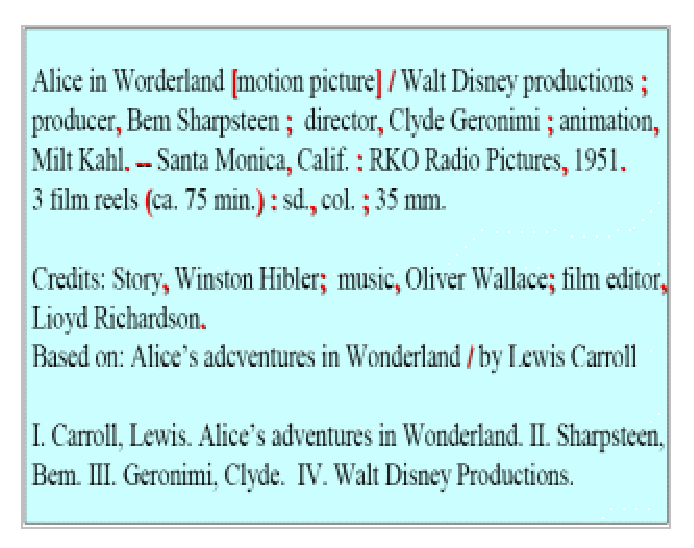
\includegraphics[width=0.7\textwidth]{aacr2}
\caption{Ficha catalográfica considerando as recomendações AACR2}
\label{fig:aacr2}
\end{figure}

Percebe-se que as descrições são para especialistas na área de catalogação e são feitas com domínio sobre os formatos e sobre as regras de classificação associadas. Um exemplo de catalogação na banda três está apresentado na figura \ref{fig:marc2}, com a descrição de um registro no formato MARC, de uso comum por profissionais da área da Biblioteconomia.

\graphicspath{{figuras/}}
\begin{figure}[H]
\centering
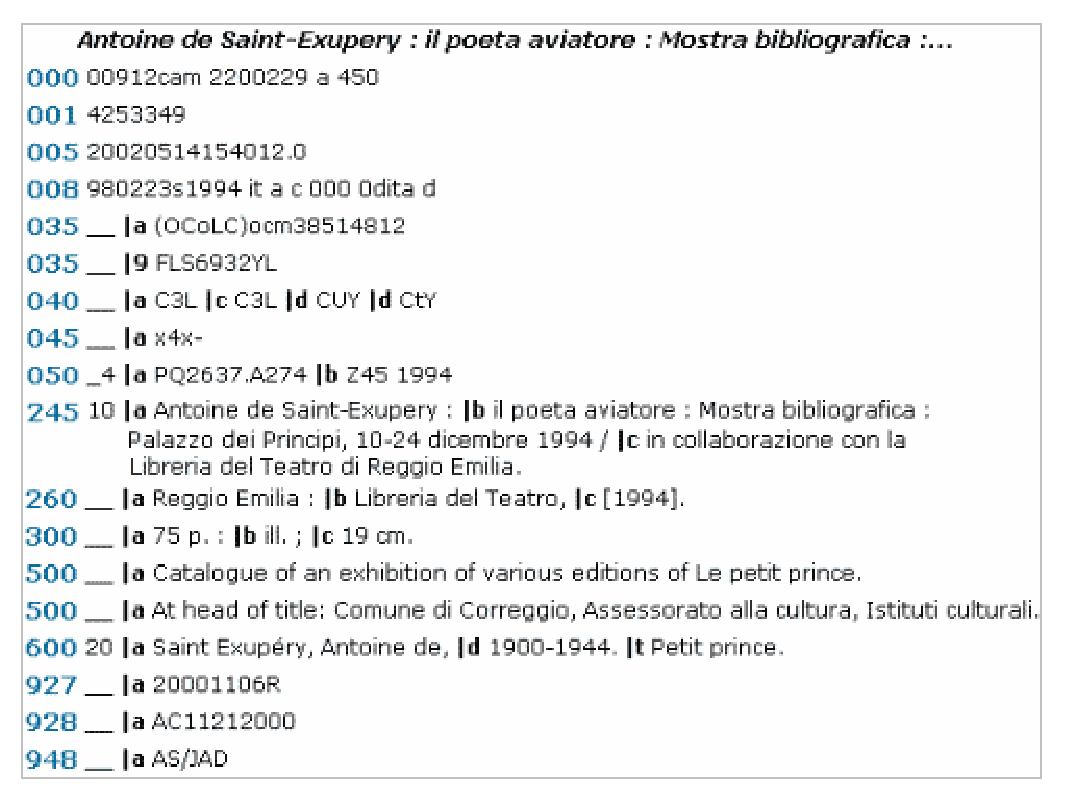
\includegraphics[width=0.7\textwidth]{marc2}
\caption{Exemplo de descrição bibliográfica em formato MARC}
\label{fig:marc2}
\end{figure}

O Dublin Core é interessante porque envolve um conjunto de dados padronizados para descrição de recursos na web. Caracteriza-se por sua utilidade e flexibilidade na representação dos dados e contém 15 elementos na sua composição básica, conforme exemplo descrito na figura \ref{fig:exdublincore}. Esse padrão é acordo conceitual sobre termos de fácil uso e não necessita ser especializado no processo de catalogação para descrição dos recursos na web.

\graphicspath{{figuras/}}
\begin{figure}[H]
\centering
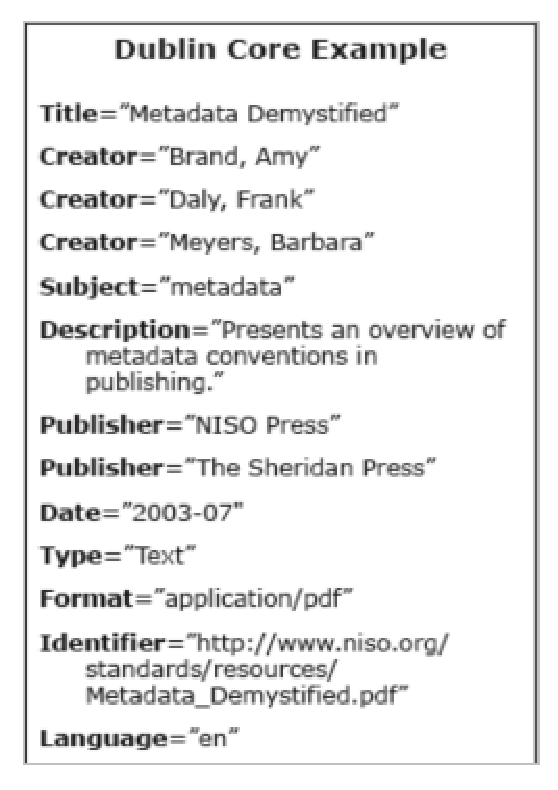
\includegraphics[width=0.5\textwidth]{exemplo_dublincore}
\caption{Exemplo de escrição bibliográfica em formato Dublin Core}
\label{fig:exdublincore}
\end{figure}

\section{Ferramentas de Biblioteca Digital}

Aqui são descritas as principais ferramentas de biblioteca digital

\subsection{Greenstone} 

Greenstone é um conjunto de softwares para a construção e distribuição de coleções de bibliotecas digitais. Ele organiza a informação, publicando-a na Internet ou em CD-ROM. Greenstone é produzido pela Universidade de Waikato, desenvolvido e distribuído em cooperação com a \textit{UNESCO} e a \textit{ONG Human Info}. É um software \textit{open-source}, multilinguagem e emitido nos termos da GNU.
 
O objetivo do software Greenstone é capacitar os usuários, especialmente em universidades, bibliotecas e outras instituições de serviço público, para construir suas próprias bibliotecas digitais. Através de \textit{plugins}, o Greenstone pode importar documentos digitais em formatos de texto incluindo HTML, JPG, TIFF, MP3, PDF, vídeo, Textos, PDF, HTML e documentos similares são convertidos em \textit{Greenstone Archive Format} (GAF), que é um formato XML equivalente.

\subsection{KEA}

KEA\footnote{Maiores informações disponíveis em: \url{http://www.nzdl.org/Kea}} é um algoritmo para extração de frases a partir de documentos de texto. Ele pode ser usado para indexação livre ou para a indexação com um vocabulário controlado. Entre outras características, o KEA possui várias versões, é implementado em Java\footnote{Maiores informações em: \url{http://www.java.com}} e é independente de plataforma. Além disso, é um software \textit{open-source} distribuído sob a licença GNU \footnote{Informações em: \url{http://www.gnu.org}}.

No KEA palavras/frases-chave são amplamente utilizadas em grandes coleções de documentos. Elas descrevem o conteúdo dos documentos e fornecem uma espécie de metadados semânticos úteis para uma grande variedade de propósitos. A tarefa de atribuir frases-chave a um documento é chamada de indexação \textit{keyphrase}. Por exemplo, trabalhos acadêmicos são frequentemente acompanhados por um conjunto de frases livremente escolhidas pelo autor. Em bibliotecas, indexadores profissionais selecionam frases-chave de um vocabulário controlado (também chamado \textit{Subject Headings}) de acordo com regras da catalogação definida. Na Internet, bibliotecas digitais, ou qualquer outro depósito de dados também usam frases (\textit{tags} ou etiquetas de conteúdo) para organizar e proporcionar um acesso temático aos seus dados.


\subsection{Omeka}
\label{sub:omeka}

Omeka\footnote{Disponível em \url{http://www.omeka.org}} é uma plataforma para disponibilização e manutenção de  bibliotecas digitais bem flexível, isto é, ele se adapta muito bem para sua finalidade, seja ele museu, biblioteca de imagens, livros, lugares (bibliotecas sobre guerras), entre outros. O Omeka é um software livre, com código aberto e escrito em PHP \footnote{Disponível em: \url{http://www.php.net}}. Sua instalação é bastante simples, bastando apenas que a máquina do cliente possua o PHP 5 instalado, juntamente com o banco de dados MySQL\footnote{Disponível em: \url{http://www.mysql.org}} e um servidor HTTP (como o \textit{Apache}\footnote{Informações em: \url{http://www.nginx.org}} ou \textit{nginx}\footnote{Maiores Informações: \url{http://www.nginx.org}}). O Omeka não possui uma finalidade específica como o GreenStone, Dspace, entre outros. Na Figura \ref{fig:finalidadeomeka} podemos visualizar que o Omeka caminha na intersecção de três ferramentas, entre elas: Sistema de gerenciamento de conteúdo (\textit{Web Content Management} ou CMS\footnote{Maiores Informações em: \url{http://pt.wikipedia.org/wiki/Sistema_de_gerenciamento_de_conte\%C3\%BAdo}}), Repositório de arquivos digitais e coleções (biblioteca digital) e sistemas para gerenciamento de museus.

\graphicspath{{figuras/}}
\begin{figure}[H]
\centering
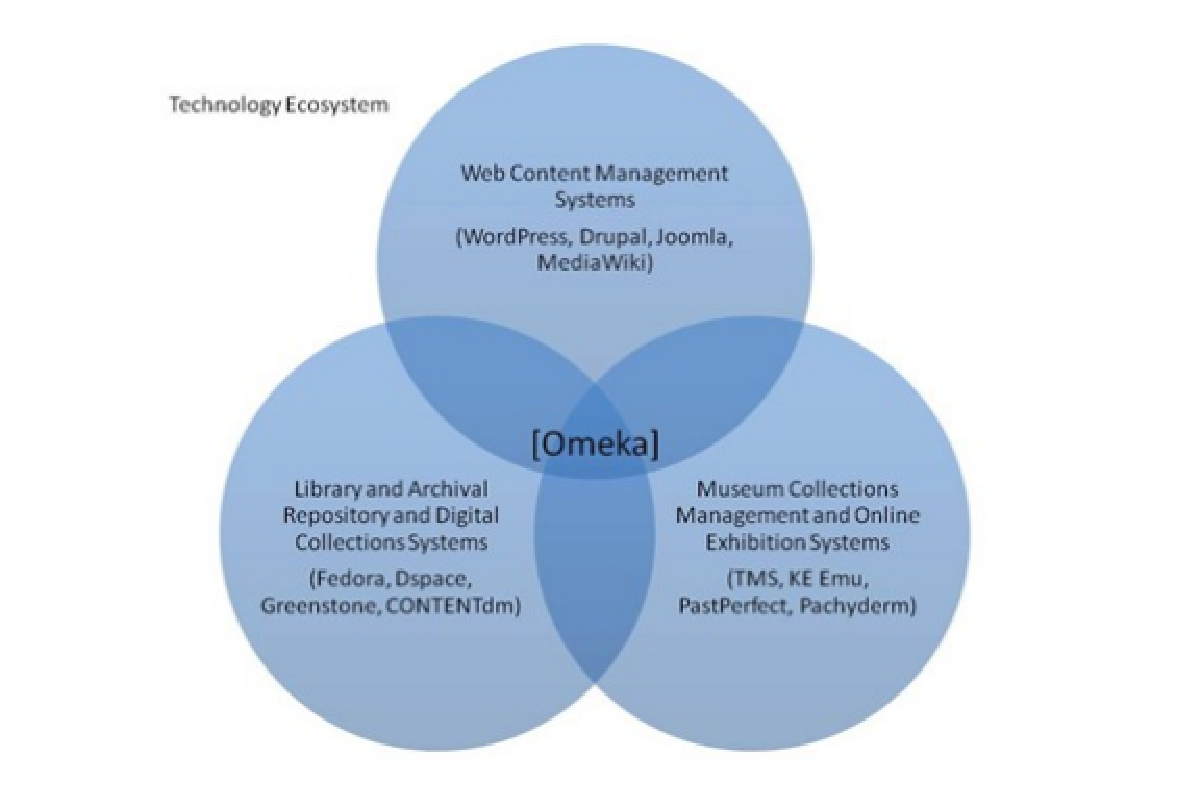
\includegraphics[width=0.7\textwidth]{finalidade_omeka}
\caption[Finalidade do Omeka]{Finalidade do Omeka. Retirado do Site \url{http://www.omeka.org}}
\label{fig:finalidadeomeka}
\end{figure}
%Figura A.2: Finalidade do Omeka Retirado de OMEKA.ORG

O Omeka possui uma interface muito intuitiva e de fácil personalização, isso se deve ao fato de ser construído para pessoas que não são experientes na utilização de computadores. Diferentemente do GreenStone, o Omeka não possui uma interface offline para inserção de dados, já que todas as funções são realizadas dentro do site.

O Omeka possui uma interface muito intuitiva e de fácil personalização, isso se deve ao fato de ser construído para pessoas que não são experientes na utilização de computadores. Diferentemente do GreenStone, o Omeka não possui uma interface offline para inserção de dados, já que todas as funções são realizadas dentro do site. Sua arquitetura possui o padrão MVC (\textit{Model-View-Controller}) que foi visto na seção \ref{sub:arquiteturamvc}.

Outro padrão arquitetural que o Omeka possui é sua extensibilidade. Ou seja, podemos estender temas ou \textit{plugins} desenvolvidos pela comunidade ou por nós, de forma bastante simples: basta colocar o tema dentro da pasta \textit{/themes} (a partir da raiz do Omeka), ou no caso de um \textit{plugin}, existe uma pasta /\textit{plugins}, onde estão localizados todos os \textit{plugins}. Após esse passo, basta logar como administrador na interface do Omeka e ativar os \textit{plugins} ou o tema. Mais detalhes de extensibilidade é visto na seção \ref{sub:arquiteturaplugin}.

Uma das vantagens do desenvolvimento de uma arquitetura extensível através de \textit{plugins} é que novas funcionalidades podem ser incluídas sem a necessidade da interferência do desenvolvedor no código fonte do core do Omeka, uma exemplo de uma nova funcionalidade que foi incluída é a compatibilidade com o protocolo OAI-PMH. Para o desenvolvimento de \textit{plugins} e temas, o Omeka fornece toda uma documentação detalhada para o desenvolvimento.

\subsection{Simile}

Símile \footnote{Maiores informações disponíveis em: \url{http://simile.mit.edu}} é um projeto conjunto realizado pelo MIT Libraries~\footnote{Maiores informações em: \url{https://libraries.mit.edu/}}e CSAIL MIT \footnote{Disponível em: \url{http://www.csail.mit.edu/}} visando melhorar a interoperabilidade entre os ativos digitais, esquemas/vocabulários/ontologias, metadados e serviços. Um desafio fundamental é que as coleções que devem interoperar muitas vezes são distribuídas em repositórios individuais, comunitários e institucionais. Ele busca fornecer serviços ao usuário final, com base nos ativos, esquemas/vocabulários/ontologias e metadados realizada em tais repositórios. 

O Simile busca alavancar e estender o DSpace, aumentando o seu apoio a esquemas arbitrários e metadados, principalmente em aplicações de RDF e técnicas da web semântica. O projeto também visa implementar uma arquitetura de difusão digital de ativos baseados em padrões web. A arquitetura de divulgação fornece um mecanismo para adicionar “visões” úteis de um artefato digital particular (ou seja, ativos, esquema ou instância de metadados), e vincular essas opiniões aos serviços de consumo. O projeto está totalmente comprometido com os princípios de código aberto de distribuição de software e de desenvolvimento aberto. Por isso, ele libera a propriedade intelectual criada (software e relatórios) sob uma licença do tipo BSD.
 
\subsection{JeromeDL}

JeromeDL\footnote{Disponível em: \url{http://www.jeromedl.org}.}  é uma Biblioteca Digital Semântica Social. Como uma biblioteca digital, permite às instituições facilmente publicarem documentos na web. Ela suporta uma variedade de formatos de documentos e permite armazenar e consultar uma rica descrição bibliográfica de cada documento. Para encontrar documentos relevantes na JeromeDL os usuários podem usar recursos de pesquisa e navegação. O sistema permite a pesquisa por texto completo, por metadados específicos tais como autor ou ano de publicação. Além disso, os usuários também podem encontrar o conteúdo de documentos pela navegação através das categorias de assunto e também por palavras-chave.

Com os serviços do JeromeDL, cada usuário da biblioteca pode marcar livros interessantes, artigos ou outros materiais em diretórios semanticamente anotados. Os usuários podem permitir que outros vejam seus bookmarks e anotações e compartilhar seus conhecimentos dentro de uma rede social. O JeromeDL também pode também tratar um simples recurso de biblioteca como uma postagem de e-mail em um blog. Dessa forma, os usuários podem comentar o conteúdo do recurso e responder aos comentários dos outros e desta forma criar novos conhecimentos.

\subsection{DSpace}

DSpace\footnote{Informações adicionais em: \url{http://www.dspace.org/}.} é um software de código fonte aberto que fornece facilidades para o gerenciamento de acervo digital, utilizado para implementação de repositórios institucionais. Suporta uma grande variedade de tipo de documentos, tais como: livros, teses e dissertações, fotografias, filmes, áudio, e outros. Os documentos são organizados em comunidades e coleções.

O DSpace é disponibilizado livremente às instituições de investigação, sob a forma de um produto de código aberto, que pode ser livremente adaptado e expandido funcionalmente, nos termos da BSD \textit{Open source license}. Suas possibilidades de uso incluem: (i) capturar e descrever documentos digitais de acordo com um \textit{workflow} adaptável aos processos específicos de uma comunidade, (ii) distribuir os documentos digitais da instituição na Web, possibilitando a pesquisa e obtenção de cópias aos utilizadores, e (iii) preservar os documentos digitais a longo prazo.

O DSpace aceita todas as formas de materiais digitais, incluindo arquivos de texto, imagem, vídeo e áudio, o que possibilita custodiar os mais variados tipos de conteúdos, tais como, livros, artigos, relatórios técnicos, \textit{working papers}, artigos de conferências, e-teses, conjuntos de dados (estatísticos, geoespaciais, etc.), programas de computador, modelos e simulações visuais, etc. Como forma de se adaptar às necessidades específicas de cada instituição e dos seus departamentos, as possibilidades de “customização” do DSpace incluem, não só, a definição de \textit{workflows “à medida”}, mas também, a especificação de regras de utilização e formatos digitais suportados.

O DSpace permite a aplicação de variadas técnicas que garantam a segurança dos documentos digitais submetidos ao repositório. Algumas destas técnicas consistem na realização de cópias de segurança, espelhamento e atualização da infra-estrutura física (i.e., a migração de um suporte físico obsoleto para outro mais atual). Além disso, a cada item é atribuído um identificador único de forma a assegurar a sua recuperação na ocorrência de uma migração de dados.

O repositório do MIT conta com um mecanismo de aconselhamento aos fornecedores de conteúdos para que a documentação depositada seja fornecida nos formatos mais adequados à sua preservação em longo prazo. Os administradores de cada comunidade têm a possibilidade de limitar o acesso aos conteúdos, quer ao nível do item submetido, quer ao nível da coleção. Para a pesquisa e recuperação dos itens, o processo de submissão de documentos ao DSpace permite a sua descrição usando uma versão qualificada do vocabulário de metadados Dublin Core.

O DSpace foi desenvolvido em linguagem Java e é suportado por um conjunto de ferramentas de código aberto (\textit{open source}), tais como: PostgreSQL\footnote{Informações em: \url{http://www.postgresql.org/}} , Tomcat\footnote{Disponível em: \url{http://tomcat.apache.org/}} e o Lucene (motor de pesquisa)\footnote{Maiores Informações: \url{http://lucene.apache.org/}}. Outros softwares necessários são o Maven\, ant\footnote{Informações em: \url{http://ant.apache.org/}} e ant-optionals\footnote{Maiores infomações em: \url{mvnrepository.com/artifact/ant/ant-optional}}.


